\documentclass[tikz,border=10pt]{standalone}
\usetikzlibrary{angles,quotes}
\begin{document}
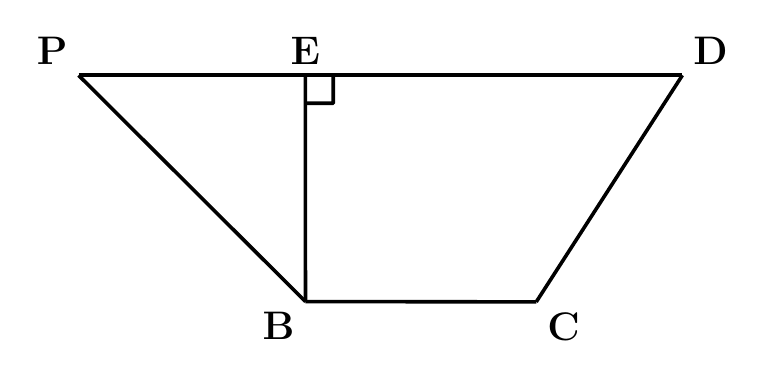
\begin{tikzpicture}[line width=1.3pt, line join=round]
\coordinate (B) at (-0.980,-1.419);
\coordinate (C) at (1.951,-1.423);
\coordinate (D) at (3.807,1.455);
\coordinate (P) at (-3.862,1.455);




\coordinate (E) at (-0.982,1.455);


\draw (P) -- (E);
\draw (E) -- (D);


\draw (P) -- (B);
\draw (B) -- (C);
\draw (C) -- (D);


\draw (E) -- (B);


\draw pic[draw, angle radius=0.355cm] {right angle=D--E--B};


\node[above left,  font=\fontsize{14}{16.8}\selectfont] at (P) {$\mathbf{P}$};
\node[above,       font=\fontsize{14}{16.8}\selectfont] at (E) {$\mathbf{E}$};
\node[above right, font=\fontsize{14}{16.8}\selectfont] at (D) {$\mathbf{D}$};
\node[below right, font=\fontsize{14}{16.8}\selectfont] at (C) {$\mathbf{C}$};
\node[below left,  font=\fontsize{14}{16.8}\selectfont] at (B) {$\mathbf{B}$};
\end{tikzpicture}
\end{document}
